%---------------------------------------------------
% Differentiation
%---------------------------------------------------
\chapter[Differentiation]{Differentiation}


\begin{figure}[h]\begin{center}
		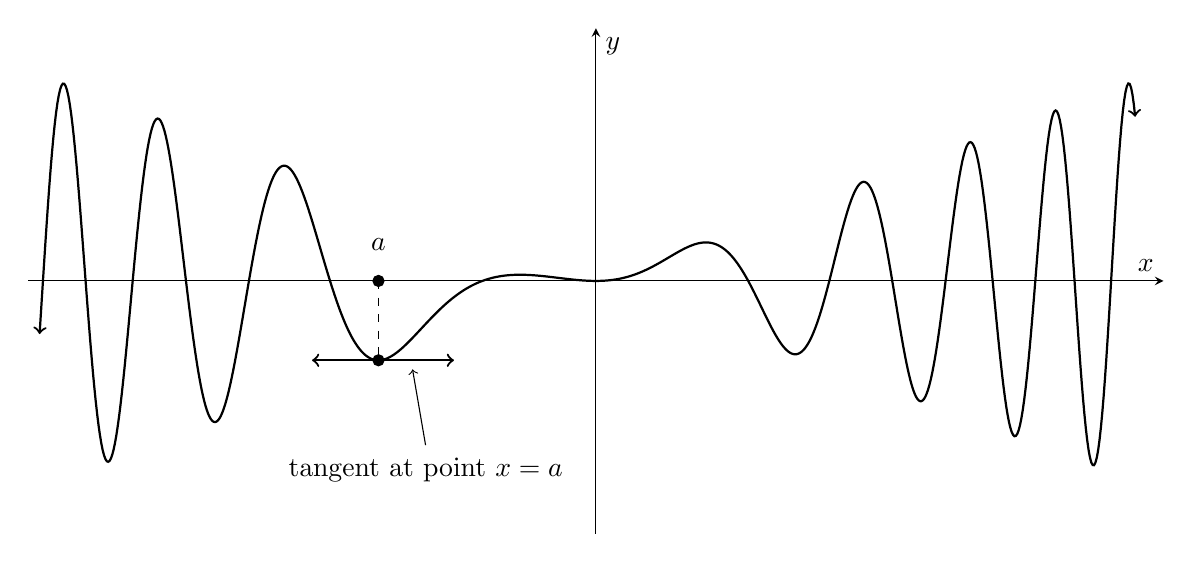
\begin{tikzpicture}
		\begin{axis}[
		axis lines=center,
		width=16cm,height=8cm,
		ymax=6,ymin=-6,
		xmax=5,xmin=-5,
		xtick=\empty,ytick=\empty,
		xlabel=$x$,ylabel=$y$,
		]
		\addplot [<->,domain=-4.9:4.75,thick, samples=800, black] {x*sin(deg(x+x^2))};
		\addplot[mark=*] coordinates {(-1.915,-1.884)};
		\addplot[<->,domain=-2.5:-1.25, thick,samples=50, black]{-1.884};
		\addplot[mark=*] coordinates {(-1.915,0)};
		\node[anchor=south] at (axis cs:-1.915,0.5) {$a$};
		\node[anchor=south] at (axis cs:-1.5,-5) {tangent at point $x=a$};
		\draw[<-](axis cs:-1.615,-2.1)--(axis cs:-1.5,-3.9);
		\draw[dashed](axis cs:-1.915,0)--(axis cs:-1.915,-2);
		\end{axis}
		\end{tikzpicture}
		\caption{The function is smooth everywhere; there are no gaps or sharp transitions, and therefore it has a well defined tangent line at any point. One of these tangents is shown at $x=a$. The function that defines \textit{all} possible tangents is called the derivative.}\end{center}
\end{figure}

\vspace{1cm}
Before sharpening our pencil consider the \href{https://calculusmadeeasy.org/prologue.html}{Prologue} to a book titled ``\emph{Calculus Made Easy\footnote{The full and verbose title: Calculus Made Easy: Being a Very-Simplest Introduction to Those Beautiful Methods of Reckoning Which are Generally Called by the Terrifying Names of the Differential Calculus and the Integral Calculus.}}" by Silvanus P. Thompson published in 1910:

\begin{quotation}
	Considering how many fools can calculate, it is surprising that it should be thought either a difficult or a tedious task for any other fool to learn how to master the same tricks.

	Some calculus-tricks are quite easy. Some are enormously difficult. The fools who write the textbooks of advanced mathematics — and they are mostly clever fools — seldom take the trouble to show you how easy the easy calculations are. On the contrary, they seem to desire to impress you with their tremendous cleverness by going about it in the most difficult way.

	Being myself a remarkably stupid fellow, I have had to unteach myself the difficulties, and now beg to present to my fellow fools the parts that are not hard. Master these thoroughly, and the rest will follow. What one fool can do, another can.
\end{quotation}
\clearpage
Thompson goes on to describe the differential operator, `d':

\begin{quotation}
	The preliminary terror, which chokes off most fifth-form boys from even attempting to learn how to calculate, can be abolished once for all by simply stating what is the meaning–in common-sense terms–of the two principal symbols that are used in calculating.

	These dreadful symbols are:\medskip

	(1) \textbf{d} which merely means “a little bit of.”\medskip

	Thus d$x$ means a little bit of $x$; or d$u$ means a little bit of $u$. Ordinary mathematicians think it more polite to say “an element of,” instead of “a little bit of.” Just as you please. But you will find that these little bits (or elements) may be considered to be indefinitely small.
\end{quotation}

For the second symbol, the integrand, $\int$, you will have to jump to the next Chapter.\\
\rule{\textwidth}{0.4pt}

\section*{Rate of Change}
We will begin with the concept of average speed. If you travel a distance of 120 km in 2 hours then your average speed is 60 kph.
\begin{center}
Average speed $ =\displaystyle\frac{\text{distance travelled}}{\text{time elapsed}}$
\end{center}\par
A distance/time graph can be drawn. The average speed can be expressed using function notation
\begin{center}
Average speed $\displaystyle =\frac{s (b) -s (a)}{b -a}$
\end{center}\par
Finding the average rate of change is important in many contexts and in fact the average rate of change can be defined for any function.

The average rate of change of the function $\displaystyle y =f (x)$ is $\displaystyle\frac{\text{change in }y}{\text{change in }x}$ or $\displaystyle\frac{f (b) -f (a)}{b -a}$\hfill(1)

The average rate of change is the slope of the \textbf{secant line} between $x =a$ and $x =b$ on the graph of $f$,\ that is the slope of the line that passes through $(a ,f (a))$ and $(b ,f (b))$.
\clearpage
\example Calculate the average rate of change for the function $f (x) =x^{2} +4$ between the following points:
\begin{tasks}(3)
\task $x =2$ and $x =6$ \\
\solution\\ Using the function notation in (1) above, \[\frac{f(2)-f(6)}{2-6}=\frac{8-40}{-4}=8\]

\task $x =5$ and $x =10$ \\
\solution\\
\[\frac{f(5)-f(10)}{5-10}=\frac{29-104}{-5}\]
\[=15\]

\task $x =a$ and $x =a +h$\\ ($h \neq 0$) \\
\solution\\
\[\frac{f(a)-f(a+h)}{a-(a+h)}\]
\[=\frac{a^2+4-([a+h]^2+4)}{-h}\]
Can this be simplified further?
\end{tasks}
\begin{figure}\begin{center}
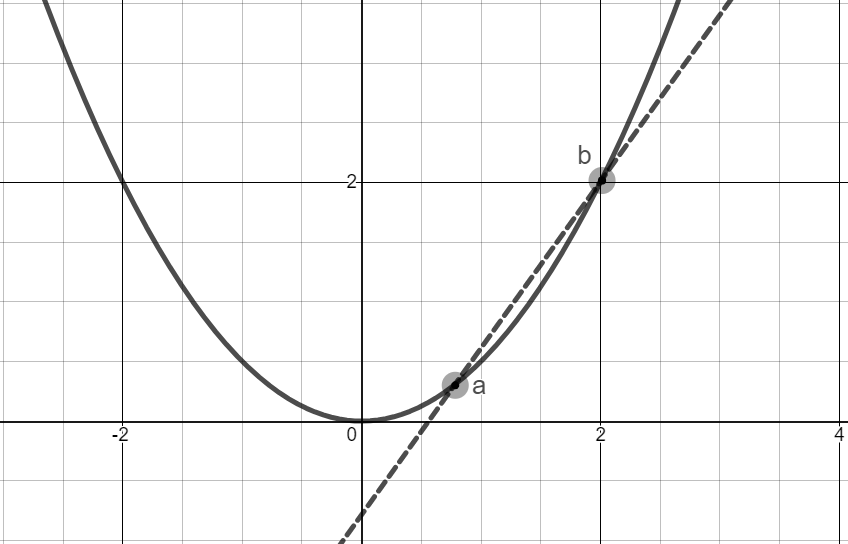
\includegraphics[width=12cm]{secant}
\caption{As the two points come closer together the secant line $ab$ gets shorter. When $b$ is at $a$ the secant line becomes a tangent line. See this \href{https://www.desmos.com/calculator/1zlwbppkuh}{animated with Desmos} (check the link on blackboard).}\end{center}
\end{figure}

%---------------------------------------------------
% tangents
%---------------------------------------------------
\subsection*{Tangents}
We now investigate the process of changing the value of $(b -a)$ in formula (1) the slope of the secant approaches the slope of the tangent at $x =a$. However, as $b -a$ is made smaller and smaller, eventually it will get to zero. This is necessary to find the exact tangent, except now the denominator of equation (1) is zero! A new definition can help us avoid this \textit{math error}.
\begin{tcolorbox}
\textbf{Definition:} The tangent line to the curve $y =f (x)$ at the point $P (a ,f (a))$ is the line through $P$ with slope \[m =\Lim{x\to a}\frac{f (x) -f (a)}{x -a}\] provided that the \textit{limit} exists. $\Lim{x\to a}$ is the ``limit as $x$ approaches $a$.''
\end{tcolorbox}
This means that as the value of $x$ gets close to $a$ the function remains smooth. Imagine zooming in on a function, from far away it may appear smooth, but up close it could have some gaps or discontinuities.  Limits do not exist at sharp transitions in a graph, or where the function does not exist (think of piecewise functions).

We sometimes refer to the slope of the tangent line to a curve at a point as the slope of the curve at that point. The idea is that if we zoom in far enough towards the point then the curve looks almost like a straight line. The more we zoom in the more the parabola looks like a straight line.

\begin{figure}\begin{center}
		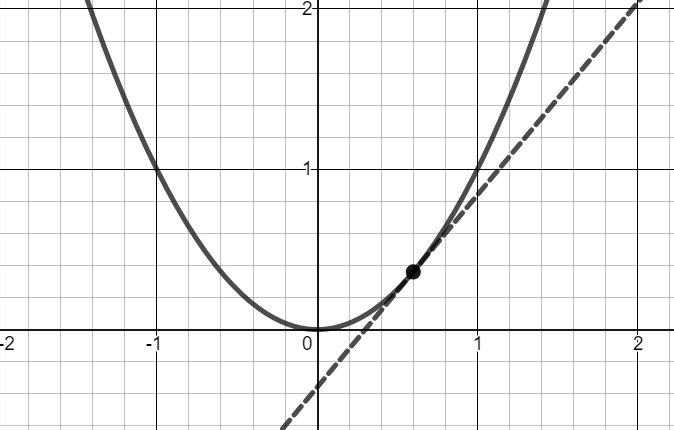
\includegraphics[width=12cm]{secant2tangent}
		\caption{A tangent can only touch the curve once. The slope of the tangent is perpendicular to the radius at the tangent point. This slope is called the rate of change or \textit{derivative} of the function at the point. See this \href{https://www.desmos.com/calculator/ialy1tknoo}{animated with Desmos} (check the link on blackboard).}\end{center}
\end{figure}

Using function notation for the tangent line is usually easier to use and is often preferred. The slope of the secant line between $x =a$ and $x =a +h$ is $\displaystyle \frac{f (a +h) -f (a)}{h}$. This looks familiar from \textsc{example} 3 above. We can now use this as a definition:

\begin{tcolorbox}
$$\text{slope }=m=\Lim{h\to 0} \frac{f(a+h)-f(a)}{h}$$
\end{tcolorbox}
This is limit notation, $\Lim{h\to 0} $, and we would say `the limit as $h$ approaches $0$'. Note that if $h=0$ the function is now undefined (math error). So $h$ is allowed to get close to zero, but not actually equal zero.



%---------------------------------------------------
% Derivatives from 1st Principles
%---------------------------------------------------
\section{Derivatives from 1st Principles}
Because the expression $\Lim{h \to 0}\frac{f (a +h) -f (a)}{h}$ occurs so widely it is given a special name and notation.

The derivative of a function at a number $a$, denoted by $f^{ \prime } (a)$ is
\begin{tcolorbox}
Definition of the derivative:\qquad$\displaystyle f^{ \prime } (a) =\Lim{h \to 0}\frac{f (a +h) -f (a)}{h}$
\end{tcolorbox}

The process of finding the derivative using the above definition is called finding the derivative \textit{from first principles}. So far we have found a derivative of a function $f$ at a fixed number $a$. If we replace $a$ in this equation with a variable $x$ we obtain
\[f^{ \prime } (x) =\Lim{h \to 0}\frac{f (x +h) -f (x)}{h}\tag*{*Note the difference from above}\]
given any number $x$ for which this limit exists. We assign to $x$ the number $f^{ \prime } \left (x\right )$. So we can regard $f^{ \prime }$ as a new function which we call the derived function or the derivative of $x$.

\subsection*{Derivatives of Polynomial Functions}
The constant function $f (x) =c$ is considered a polynomial of degree zero. Using the method of first principles we can find the derivative as follows:
$$f^{ \prime } (x) =\Lim{h\to 0}\frac{f (x +h) -f (x)}{h} =\Lim{h\to 0}\frac{c -c}{h} =\Lim{h\to 0}0 =0$$

\subsection*{Higher Power Polynomials}
When $f (x) =x$ it can be shown from first principles that $f^{ \prime } (x) =1$. Similarly when $f (x) =x^{2\text{}}$it can be shown that $f^{ \prime } (x) =2 x$ and when $f (x) =x^{3}$ it can be shown that $f^{ \prime } (x) =3 x^{2}$.

\example Find $f'(x)$ for $f (x) =x^{4}$ from first principles.

\solution \begin{align*}f^{ \prime } (x) &  = \Lim{h\to 0}\frac{f (x +h) -f (x)}{h} \\
 &  = \Lim{h\to 0}\frac{(x +h)^{4} -x^{4}}{h} \\
 &  = \Lim{h\to 0}\frac{x^{4} +4 x^{3} h +6 x^{2} h^{2} +4 x h^{3} +h^{4} -x^{4}}{h} \\
 &  = \Lim{h\to 0}\frac{4 x^{3} h +6 x^{2} h^{2} +4 x h^{3} +h^{4}}{h} \\
 &  = \Lim{h\to 0}(4 x^{3} +6 x^{2} h +4 x h^{2} +h^{3})\text{ here, substitute }h=0 \\
 f'(x)&  = 4 x^{3}\end{align*}

This pattern will follow for any similar polynomial: If $f (x) =x^{n}$ then $f^{ \prime } (x) =n x^{n -1}$. Or alternatively
\begin{tcolorbox}
The Power Rule for Differentiation:\qquad$\displaystyle \frac{d}{d x} (x^{n}) =n x^{n -1}$
\end{tcolorbox}

This pattern implies that $n$ must be a positive integer. It can be shown that from the definition of a derivative $\frac{d}{d x} \genfrac{(}{)}{}{}{1}{x} = -\frac{1}{x^{2}}$ or $y =x^{ -1}$ then $\frac{d y}{d x} = -1 \times x^{ -2}$, which proves the power rule for $n = -1$.

Similarly if the exponent is a fraction it can be shown that the power rule holds e.g. if $f (x) =\sqrt{x}$ then $f^{ \prime } (x) =\frac{1}{2 \sqrt{x}}$ or $f (x) =x^{\frac{1}{2}}$ then $f^{ \prime } (x) =\frac{1}{2} x^{ -\frac{1}{2}}$. It can be shown that the power rule holds for any real number $n$.

\subsection*{The Natural Exponential Function}
Recall the natural exponential function from section~\ref{sec:naturalExponential}. Here we can see why precisely it is so special. Using limit notation, we can say that $e$ is the number such that $\Lim{h\to 0}\frac{e^{h} -1}{h} =1$. The derivative is:

\begin{tcolorbox}
The Derivative of the Natural Exponential Function
$$\frac{d}{d x} \left (e^{x}\right ) =e^{x}$$
\end{tcolorbox}

The natural exponential function is unique because \textbf{it has its own derivative!} Geometrically this means that the slope of the tangent at any point is the same as the y-coordinate, $f(x)$, of that point.

%---------------------------------------------------
% Standard Derivatives
%---------------------------------------------------
\section{Standard Derivatives}
The basic functions have easily repeatable patterns to find their derivatives. The common ones are summarized in the table below:
% have to see how the array stretch looks
\renewcommand\arraystretch{1.2}
\begin{center}
	\begin{tabular}{ccll}
		\toprule
		Function& Derivative&&Notes\\
		$f(x)$ & $f'(x)$  &&\\ \midrule
		$A$&0&&$A$ is constant\\
		$x$&$1$&&power rule for $x^1$\\
		$Ax$&$A$&&$A$ is a constant multiple\\ \midrule
		$x^n$ & $nx^{n-1}$ &&power rule - general form\\
		$e^x$ & $e^x$  && exponential\\
		$\ln(x)$ & $\frac{1}{x}$ &&logarithmic\\ \midrule
		$\sin(x)$ & $\phantom{-}\cos(x)$  && trigonometric\\
		$\cos(x)$ & $-\sin(x)$ && \\
		$\tan(x)$ & $\phantom{-}\sec^2(x)$ && \\ \bottomrule
	\end{tabular}
\end{center}\clearpage
\example Find the following derivatives:
\begin{tasks}[after-item-skip=3ex](3)
	\task $f(x)=7$\\ 7 is constant (no variables: `$x$'), so $f'(x)=0$
	\task $f(x)=7x$\\ 7 is a constant multiple: \\ $f'(x)=7$
	\task $f=7x^2$\\ using the power rule:\\ $f'=7(2)x^1=14x$
	\task $f(x)=\pi x^{-3}$\\pi is a constant:\\ $f'(x)=-3\pi x^{-4}$
	\task $\displaystyle g(x)=x^{\frac{3}{4}}$\\ use the power rule for fractional exponents:\\ $\displaystyle g'(x)=\frac{3}{4}x^{-\frac{1}{4}}$
	\task $f(x)=\displaystyle\frac{e^x}{3}$\\ the exponential always has its own derivative, $\frac{1}{3}$ is a constant: $f'(x)=\frac{1}{3}e^x$
	\task $s(t)=2\sin t$\\ 2 is a constant: \\$s'(t)=2\cos t$
	\task $f=\displaystyle\frac{\cos r}{3}$\\ $\frac{1}{3}$ is a constant:\\ $f'=-\frac{1}{3}\sin r$
	\task $f(x)=\tan (\pi x)$\\ this requires the Chain Rule (\ref{sec:chainRule}): $f'(x)=\pi\sec^2 (\pi x)$
\end{tasks}

%---------------------------------------------------
% max, min and tangents
%---------------------------------------------------
\section{Maximums, Minimums, and Tangents}
Turning points occur at the boundary between regions in a function.  A function that transitions from increasing to decreasing must have a turning point. In the function below, $f(-1)=2$ means the point $(-1,2)$ is a turning point. More specifically this is a local maximum of our function. It is the highest point in its \emph{local} neighbourhood. Notice that the other boundary has different properties: it is the lowest point. So $f(1)=-2$ means the point $(1,-2)$ is a local minimum.
\begin{multicols}{2}
The boundary means that the slope of the \textit{tangent} has gone from increasing to decreasing. Or from positive to negative. During this transition it had to go through zero, and so a turning point can be found anywhere the slope is equal to zero: $f'(x)=0$. Remember that the first derivative represents the slope of the function.\medskip\\
\example Find the turning points for \[f(x)=x^3-3x\]
\columnbreak
	\begin{center}
		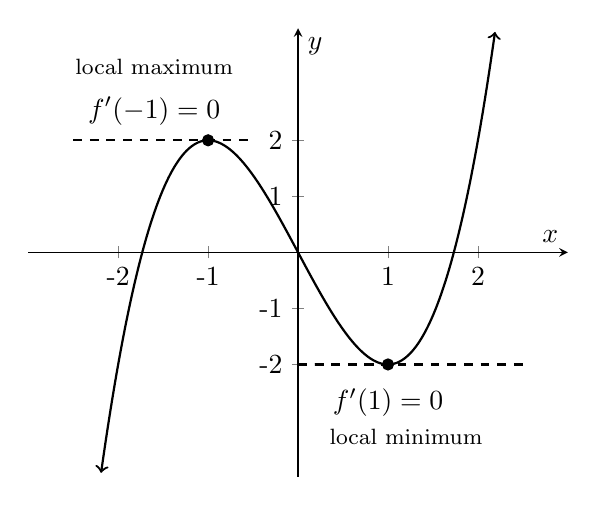
\begin{tikzpicture}\label{fig:maxMin}
		\begin{axis}[
		axis lines=center,
		ymax=4,ymin=-4,
		xmax=3,xmin=-3,
		xtick={-2,...,2},xticklabels={-2,-1,0,1,2},
		ytick={-2,...,2},yticklabels={-2,-1,0,1,2},
		xlabel=$x$,ylabel=$y$,
		]
		\addplot [<->,domain=-2.19:2.19,thick, samples=200, black] {x^3-3*x};
		\addplot [dashed,domain=0:2.5,thick, samples=200, black] {-2};
		\addplot [dashed,domain=-2.5:-0.5,thick, samples=200, black] {2};
		\addplot[mark=*] coordinates {(1,-2)};
		\addplot[mark=*] coordinates {(-1,2)};
		\node[anchor=south] at (axis cs:1,-3.1) {$f'(1)=0$};
		\node[anchor=south] at (axis cs:1.2,-3.6) {\footnotesize{local minimum}};
		\node[anchor=south] at (axis cs:-1.6,2.1) {$f'(-1)=0$};
		\node[anchor=south] at (axis cs:-1.6,3) {\footnotesize{local maximum}};
		\end{axis}
		\end{tikzpicture}
	\end{center}
\end{multicols}
\begin{multicols}{2}
\solution Set the derivative equal to zero and solve for values of $x$.
\begin{align*}
\frac{dy}{dx}&=3x^2-3\\
0&=3x^2-3\\
3&=3x^2\\
1&=x^2\\
x&=1, \,\mathrm{ and }\, x=-1
\end{align*}
Therefore the $x-$values of the turning points are 1 and $-1$. Note there are two turning points in our function so there should be two corresponding solutions.\\
\begin{align*}
f(1)&=(1)^3-3(1)\\
&=1-3=-2
\end{align*}
Therefore $(1,-2)$ is the first turning point. Similarly, $(-1,2)$ is found as the other turning point. These are both shown in the figure above.\end{multicols}

\examq Given the cubic function $\displaystyle f(x)=2x^3-3x^2-12x+1$, find\\ \textbf{(a)} the equation of the tangent line to $f(x)$ at the point $x=-2$, and \textbf{(b)} all turning points.\medskip\\
\solution
\begin{tasks}(2)
\task Find the slope of the function at $x=-2$ by finding the derivative:
\begin{align*}
f'(x)&=6x^2-6x-12\\
f'(-2)&=6(4)-6(-2)-12=24\\
&\text{find the corresponding y-value:}\\
f(-2)&=2(-8)-3(4)+24+1=-3\end{align*}
Use the standard point-formula for an equation of a line:
\begin{align*}
y-y_1&=m(x-x_1)\\
y-(-3)&=24(x--2)\\
y=24x+45\end{align*}


\task Set the derivative equal to zero and solve for the $x$-values:
\begin{align*}
0&=6x^2-6x-12\\
0&=x^2-x-2\\
0&=(x-2)(x+1)\\
x&=2\text{, or }x=-1\\
\text{find the y-values:}&\\
f(2)&=-19\text{, and }f(-1)=8\\
\end{align*}
Therefore the two turning points are $(2,-19)$ and $(-1,8)$. Without a graph, we don't know the nature of these points -- are they concave-up or concave-down?
\end{tasks}

\subsection*{Second Derivative Test}\label{sec:2ndDerivativeTest}
Given a graph it is easy to determine if points are maxima or minima. However, the graph is not always available, so it  helps to have a test to determine if a point is a maximum or minimum.

We know first derivative represents the slope of the function. Looking at the parabola $y=x^2$ and following the function from left to right we can plot some values of the first derivative. The graph tells us that the turning point is at $(0,0)$ and is a minimum. The value of the 1st derivative is -2,-1,0,1,2 : these numbers are increasing. This trend is always true for a local minimum.

How do we test for this trend of increasing slopes? The rate of change of the \emph{slopes} is the second derivative, and if this number (at the point $(0,0)$) is positive, then the point is a minimum.

This is called the second derivative test.\\
%maybe highlight box here%
\begin{tcolorbox}
	Second Derivative Test
	\begin{itemize}
		\item If $f'(x)=0$, and $f''(x)>0$, then the point $(x,f(x))$ is a local minimum. The graph in this neighbourhood is concave up.\\
		\item If $f'(x)=0$, and $f''(x)<0$, then the point $(x,f(x))$ is a local maximum. The graph in this neighbourhood is concave down.\\
	\end{itemize}
\end{tcolorbox}

\clearpage
\example Use the second derivative test to determine if the turning point $(-1,2)$ is a maximum or minimum on the function $f(x)=x^3-3x$\\
\solution Find the second derivative and substitute the turning point.
\begin{align*}
f'(x)&=3x^2-3\\
f''(x)&=6x\\
f''(-1)&=6(-1)=-6\\
-6&<0
\end{align*}therefore the turning point $(-1,2)$ is a local maximum. Confirm by looking at the graph on page~\pageref{fig:maxMin}.

\subsection*{Points of Inflection}\label{sec:PointsOfInflection}
\begin{multicols}{2}
There is one last feature of the initial function that can be found. There is a point in between the maximum and minimum points where the change in slopes of the function change from decreasing to increasing. This is called a point of inflection. It is where the concavity of the function changes between down and up.\columnbreak
% include the plot file for
% point of inflection graph
\begin{center}
	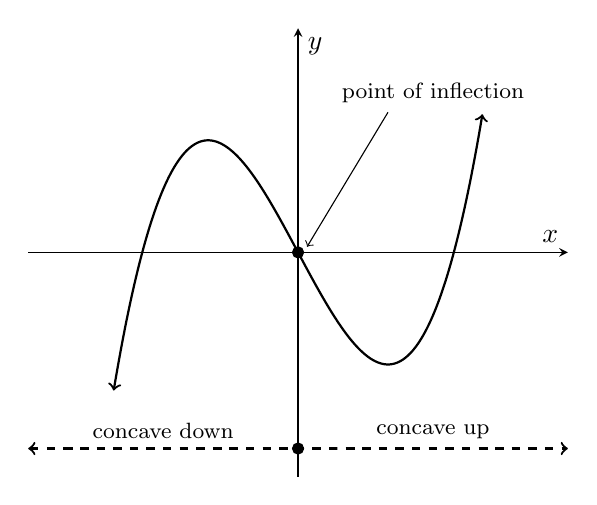
\begin{tikzpicture}
	\begin{axis}[
	axis lines=center,
	ymax=4,ymin=-4,
	xmax=3,xmin=-3,
	xtick=\empty,ytick=\empty,
	xlabel=$x$,ylabel=$y$,
	]
	\addplot [<->,domain=-2.05:2.05,thick, samples=200, black] {x^3-3*x};
	\addplot[mark=*] coordinates {(0,0)};
	\addplot[mark=*] coordinates {(0,-3.5)};
	\addplot [dashed,<->,domain=-3:3,thick, samples=200, black] {-3.5};
	\node[anchor=south] at (axis cs:1.5,-3.5) {\footnotesize{concave up}};
	\node[anchor=south] at (axis cs:-1.5,-3.5) {\footnotesize{concave down}};
	\node[anchor=south] at (axis cs:1.5,2.5) {\footnotesize{point of inflection}};
	\draw[<-](axis cs:0.1,0.1)--(axis cs:1,2.5);
	\end{axis}
	\end{tikzpicture}
\end{center}
\end{multicols}

The second derivative test can be used to determine if a function is concave-up ($>0$) or concave down ($<0$). Note there is no $=$ in these inequalities. In between is where the point of inflection can be found:
\begin{tcolorbox}
	Second Derivative Test for Concavity
	\begin{itemize}
		\item If $f''(x)=0$, then the point $(x,f(x))$ is a point of inflection.\\
	\end{itemize}
\end{tcolorbox}

%Example level: EASY
\example Find where the function changes from concave-up to concave-down.\\
\[f(x)=3x^3-12x^2+7\]
\solution Find the second derivative and set equal to zero to find the point of inflection.
\begin{multicols}{2}
\begin{align*}
f'(x)&=9x^2-24x\\
f''(x)&=18x-24\\
0&=18x-24\\
\frac{4}{3}&=x
\end{align*}
Sub back into $f(x)$ to find the $y-$value:\\
\begin{align*}
f\left(\frac{4}{3}\right)&=3\left(\frac{4}{3}\right)^3-12\left(\frac{4}{3}\right)^2+7\\
&=-7\tfrac{2}{9}
\end{align*}
Therefore, the point $\left(\tfrac{4}{3},-7\frac{2}{9}\right)$ is a point of inflection.
\end{multicols}

%---------------------------------------------------
% The Product, quotient and chain rules
%---------------------------------------------------
\section{The Product, Quotient, and Chain Rules}\label{sec:chainRule}

%-----------------------------------------------
\subsection*{The Product Rule}
Let $f (x) =x$ and $g (x) =x^{2}$. What is the derivative of $f (x) \times g (x)$? The question helps to show that the answer is NOT $f^{ \prime } (x) \times g^{ \prime } (x)$

$f (x) \times g (x) =x \times x^{2} =x^{3}$ and we know the derivative of $x^{3}$ is $3 x^{2}$. Also we know that $f^{ \prime } (x) =1$ and $g^{ \prime } (x) =2 x$ so $f^{ \prime } (x) \times g^{ \prime } (x) =1 \times 2 x =2 x$ not $3 x^{2}$.

So the derivative of the product of two functions is not the product of the derivatives of each function. In symbols this can be written
\[\left (f g\right )^{ \prime } \neq f^{ \prime } g^{ \prime }\]
\textbf{Theorem} If $f$ and $g$ are both differentiable then
\begin{tcolorbox}
	\[\frac{d}{d x} \left [f (x) g (x)\right ] =f (x) \frac{d}{d x} \left [g (x)\right ] +g (x) \frac{d}{d x} \left [f (x)\right ]\]
	\end{tcolorbox}
The Product rule is often seen in an abbreviated form as $\displaystyle \left(u v\right)^{\prime} =uv^{\prime} +vu^{\prime}$.

\example Find the derivative of $f(x)=x^2e^x$.\medskip\\
\solution Use the product rule:
$$f'(x)=(2x)(e^x)+(x^2)(e^x)$$
This could be simplified by factoring: $f'(x)=e^x(2x+x^2)$ but is not mandatory.\\\medskip
\rule{6.8cm}{0.5pt}\\
\example Differentiate $f=4\pi x\sin x$.\medskip\\
\solution Use the product rule. $4\pi$ is a constant.
$$f'=(4\pi)(\sin x)+(4\pi x)(\cos x)$$
\rule{6.8cm}{0.5pt}\\
\example If $g(x)=\frac{e^x}{3}\sqrt{x+2}$, find $g'(x)$.\medskip\\
\solution Convert the root to power form and use the product rule.
\begin{align*}
g(x)&=\frac{1}{3}e^x(x+2)^{\frac{1}{2}}\\
g'(x)&=\left[\frac{1}{3}e^x\right]\left[(x+2)^{\frac{1}{2}}\right]+\left[\frac{1}{3}e^x\right]\left[\frac{1}{2}(x+2)^{-\frac{1}{2}}\right]\\
&=\frac{e^x}{3}\sqrt{x+2}+\frac{e^x}{6\sqrt{x+2}}
\end{align*}

%-----------------------------------------------
\subsection*{The Quotient Rule}
Let $u =f (x)$ and $v =g (x)$ be differentiable functions of $x$ then we can show that
\begin{tcolorbox}
	\[\frac{d}{d x} \genfrac{[}{]}{}{}{f (x)}{g (x)} =\frac{g (x) \frac{d}{d x} \left [f (x)\right ] -f (x) \frac{d}{d x} \left [g (x)\right ]}{\left [g (x)\right ]^{2}}
\]
\end{tcolorbox}
or in abbreviated form as
\begin{equation*}\genfrac{(}{)}{}{}{u}{v}^{ \prime } =\frac{v u^{ \prime } -u v^{ \prime }}{v^{2}}
\end{equation*}
\rule{6.8cm}{0.5pt}\\
\example Differentiate with the quotient rule: $y=\frac{(s-1)(s+3)}{e^{2s}}$\medskip\\
\solution Expand the numerator first and then differentiate\\
\begin{align*}y&=\frac{s^2+2s-3}{e^{2s}}\\
y'&=\frac{(2s+2)(e^{2s})-(s^2+2s-3)(e^{2s})\cdot2}{(e^{2s})^2}\\
y'&=\frac{-2(s^2+s-4)}{e^{2s}}
\end{align*}
\rule{6.8cm}{0.5pt}\\
\example Find $f'$, given $f=\frac{\sin x}{x}$\medskip\\
\solution $$f'=\frac{[\cos(x)\cdot x]-\sin(x)}{x^2}=\frac{x\cos(x)-\sin(x)}{x^2}$$
\rule{6.8cm}{0.5pt}\\
\example Find $f'$, given $\displaystyle f=\frac{\ln x}{e^x}$\medskip\\
\solution $$f'=\frac{(\frac{1}{x})(e^x)-(\ln x)(e^x)}{e^{x^2}}$$
$$=\frac{1-x\ln x}{xe^x}$$

%-----------------------------------------------
\subsection*{The Chain Rule}
When functions are combined with other functions, they are often called composite functions. These require special treatment when differentiating.

Let $f (x) =x^{2}$ and $g (x) =2 x +1$ then $\left (f \circ g\right )$ This means $f$ `composed of' $g$ is $f \left (g \left (x\right )\right ) =f (2 x +1) =\left (2 x +1\right )^{2}$.

Also, $g$ `composed of' $f$ would be: $\left (g \circ f\right ) (x) =g \left (x^{2}\right ) =2 \left (x^{2}\right ) +1 =2 x^{2} +1$.

The differentiation rules we have met so far allow us to differentiate pairs of functions that have been added, subtracted, multiplied or divided. They do not allow us to differentiate an expression that is made from a function that is within another function.

The following are all examples of composite functions.
\begin{enumerate}
\item We can differentiate $x^{2}$ but we can't use the same procedure to differentiate $\left (1 -x\right )^{2}$. Here we can imagine if  $f (x) =x^{2}$ and $g (x) =1 -x$ then $\left (f \circ g\right ) (x) =f (1 -x) =\left (1 -x\right )^{2}$.

\item We can differentiate $\frac{1}{x^{2}}$ but we can't use the same procedure to differentiate $\frac{1}{x^{2} +1}$.

\item We can differentiate e$^{x}$ but we can't use the same procedure to differentiate $e^{x^{2}}$.
\end{enumerate}

A name often used for functions of this type is \emph{function of a function.}

Once we recognise we are dealing with a composite function we need a procedure to differentiate it. You will find that you are far more likely to be required to differentiate a composite function in a practical situation than a simple one. It can be proved that the derivative of the composite function $f \circ g$ is the product of the derivatives of $f$ and $g$. This important rule is given the name the \emph{Chain Rule}. A substitution method is often used to add clarity to the differentiation process.

Let
$y =u^{2}$ and let $u =1 -x$. Then $\frac{d y}{d u} =2 u$ and $\frac{d u}{d x} = -1$. Now $\frac{d y}{d x} =\frac{d y}{d u} \cdot \frac{d u}{d x} =2 u \times ( -1) = -2 u = -2 (1 -x) =2 (x -1)$.

The Leibniz form of the Chain Rule $\displaystyle \frac{d y}{d x} =\frac{d y}{\cancel{d u}} \frac{\cancel{d u}}{d x}$ is what gives the rule its name. Because of the apparent cancelling it is particularly
easy to learn in this form.

As an aside let us verify the rule for this example. Given
$y =(1 -x)^{2}$. We will expand the right hand side of the equation. It
becomes $y =x^{2} -2 x +1$. So $y^{ \prime } =2 x -2 =2 (x -1)$ as before.

Using function notation the Chain Rule states: If $f$ and $g$ are both differentiable and $F =f \circ g$ is the\ composite function $F (x) =f (g (x))$, then $F$ is differentiable and $F^{ \prime } =f^{ \prime } (g (x)) g^{ \prime } (x)$.

\subsection*{A Comment on the Leibniz form of the Chain Rule}
$\frac{d y}{d x} =\frac{d y}{d u} \cdot \frac{d u}{d x}$ gives the impression that the $d u$ could cancel but remember we have not defined $d u$. We have defined $\frac{d y}{d u}$ as the rate of change of $y$ with respect to $u$ and $\frac{d u}{d x}$ as the rate of change of $u$ with respect to $x$. However the apparent cancelling helps us to remember the way the differentials
are arranged. it also helps us to accept the extension of the Chain Rule to cover a function of a function of
a function etc. e.g.
\begin{align*}\text{Let }y &  = f (u)\text{, }u =g (v)\text{ and }v =h (x) \\
\text{Then }\frac{d y}{d x} &  = \frac{d y}{d u} \cdot \frac{d u}{d v} \cdot \frac{d v}{d x}\end{align*}

\example Find $F^{ \prime } (x)$ when $F (x) =\frac{1}{x^{2} +1}$. \\
\solution Using function notation $F (x) =\left (f \circ g\right ) (x) =f (g (x))$ \\
where $$f (u) =u^{ -1} \text{ and }g (x) =x^{2} +1$$
\begin{equation*}f^{ \prime } (u) = -u^{ -2}\text{and}g^{ \prime } (x) =2 x
\end{equation*}
and
\begin{align*}F^{ \prime } (x) &  = f^{ \prime } (g (x)) g^{ \prime } (x) \\
 &  = \frac{ -1}{(x^{2} +1)^{2}} \cdot 2 x \\
 &  = \frac{ -2 x}{\left (x^{2} +1\right )^{2}}\end{align*}
Using the Leibniz notation let $u =x^{2} +1$ and $y =u^{ -1}$ then
\begin{align*}F^{ \prime } (x) &  = \frac{d y}{d u} \frac{d u}{d x} = -u^{ -2} \left (2 x\right ) \\
 &  = \frac{ -1}{\left (x^{2} +1\right )^{2}} \left (2 x\right ) =\frac{ -2 x}{\left (x^{2} +1\right )^{2}}\end{align*}

To use the method we need to bring a new variable into the problem we are trying to solve. It
is recommended that you use the variable $u$ wherever possible so that you follow through using a pattern you are familiar with.

In summary: if $g$ is differentiable at $x$ and $f$ is differentiable at $g (x)$, then the composite function $F =f \circ g$ defined by $F (x) =f (g (x))$ is differentiable at $x$ and $F^{ \prime }$ is given by the product
\begin{tcolorbox}
\[F^{ \prime } (x) =f^{ \prime } [g (x)] \cdot g^{ \prime } (x)\]
\end{tcolorbox}
In Leibniz notation, if $y =f (u)$ and $u =g (x)$ are both differentiable functions, then
\begin{tcolorbox}
\[\frac{d y}{d x} =\frac{d y}{d u} \cdot \frac{d u}{d x}\]
\end{tcolorbox}

The Chain Rule will be found in many situations where functions are added, subtracted, multiplied or divided. As an example we will focus on combining the Chain Rule with the Product Rule, however any combination of these rules could be found in a problem.

\example Differentiate $\displaystyle xe^{-x^2}$.

\solution We can see that there is a product of two functions present in this example, i.e. $f (x) =x$ and $g (x) =e^{ -x^{2}}$. Also $g (x)$ is a composite function.

We have from the Product Rule
\begin{equation*}\left (f g\right )^{ \prime } =f g^{ \prime } +g f^{ \prime }
\end{equation*}

We can see that $f$, $g$ and $f^{ \prime }=1$ can be substituted immediately and only $g^{ \prime }$ requires some effort to be worked out. $g (x)$ is a composite function so $g^{ \prime } (x)$ is computed using the Chain Rule.

Let $u = -x^{2}$ then $\frac{d u}{d x} = -2 x$. Also $g (u) =e^{u}$ so $\frac{d g}{d u} =e^{u}$.
\begin{multicols}{2}
\begin{align*}\frac{d g}{d x} &  = \frac{d g}{\cancel{d u}}\cdot \frac{\cancel{d u}}{d x} \\
 &  = e^{u} \cdot  -2 x \\
 &  = e^{ -x^{2}} \cdot  -2 x \\
 &  =  -2 x\; e^{ -x^{2}} \\
\text{So }g^{ \prime } (x) &  =  -2 x\; e^{ -x^{2}}\end{align*}
Putting this all together
\begin{align*}\left (f g\right )^{ \prime } &  = f g^{ \prime } +g f^{ \prime } \\
 &  = x \cdot  -2 x\; e^{ -x^{2}} +e^{ -x^{2}} \cdot 1 \\
 &  = e^{ -x^{2}} \left [1 -2 x^{2}\right ]\end{align*}
\end{multicols}

\begin{multicols}{2}
\example Find $a'(x)$ given \\$a(x)= 4\pi x\tan (x-\frac{\pi}{4})$\medskip\\
\solution Use the product and chain rules \\
	\begin{align*}
	a'&= 4\pi\tan\big(x-\frac{\pi}{4}\big)+4\pi x\sec^2\big(x-\frac{\pi}{4}\big)(1) \\
	a'&= 4\pi\Big[xsec^2\big(x-\frac{\pi}{4}\big)+tan\big(x-\frac{\pi}{4}\big)\Big] \\
	\end{align*}
%\rule{6.8cm}{0.5pt}\\
\examq Find $\frac{dy}{dx}$ given $y=x^3e^{2x}$\medskip\\
\solution First use the product rule; there is a chain rule on 		$e^{2x}$:\begin{align*}\frac{dy}{dx}&=3x^2(e^{2x})+x^3(e^{2x})(2) \\
	\frac{dy}{dx}&=x^2e^{2x}(3+2x)\end{align*}
\end{multicols}

%---------------------------------------------------
% Parametric Differentiation
%---------------------------------------------------
\section{Parametric Differentiation}
Parametric Curves $x$ and $y$ are both given as functions of a third variable $t$ (called the \emph{parameter}). Let the equations be
\begin{equation*}x =f (t)\text{ and }y =g (t)
\end{equation*}

Each value of $t$ gives a point $(x ,y)$. As $t$ varies the point $(x ,y) =(f (t) ,g (t))$ traces out a curve in the coordinate plane called a \emph{parametric curve}. This is useful for functions that violate the vertical line test (see Section~\ref{sec:functions}) such as a circle, $x^2+y^2=r^2$, because only proper functions can be differentiated.

Both the fish and the Pokemon-looking-thingy below can be plotted using parametric equations.
\begin{figure}[H]
	\begin{subfigure}[b]{0.5\textwidth}
		\centering
		\resizebox{\linewidth}{!}{
			\begin{tikzpicture}
			\begin{axis}[
			scale=1.2,
			axis lines=center,%width=4cm,height=4cm,
			ymax=2,ymin=-2,
			xmax=2,xmin=-2,
			xtick={-2,-1.5,-1,1,2},
			xlabel=$x$,ylabel=$y$,%	ytick=\empty,
			]
			\addplot[domain=0:4*360, samples=200, thick] ({1.5*cos(x)},{-0.667*cos(1.5*x)});
			\addplot[mark=*] coordinates {(-1.5,0)};
			\addplot[mark=*] coordinates {(1.5,-0.667)};
			\draw[->,ultra thick](axis cs:1.4,0.57) -- (axis cs:1.5,0.667);
			\node[anchor=south] at (axis cs:1.5,-1.1) {$t=0$};
			\node[anchor=south] at (axis cs:-1.5,-0.8) {$t=\pi$};
			\end{axis}
			\end{tikzpicture}
		}  \caption{fish: $\displaystyle x=\frac{3\cdot\cos t}{2},\, y=-\frac{2}{3}\cos\left(\frac{3t}{2}\right)$}
	\end{subfigure}
	\begin{subfigure}[b]{0.5\textwidth}
		\centering
		\resizebox{\linewidth}{!}{
			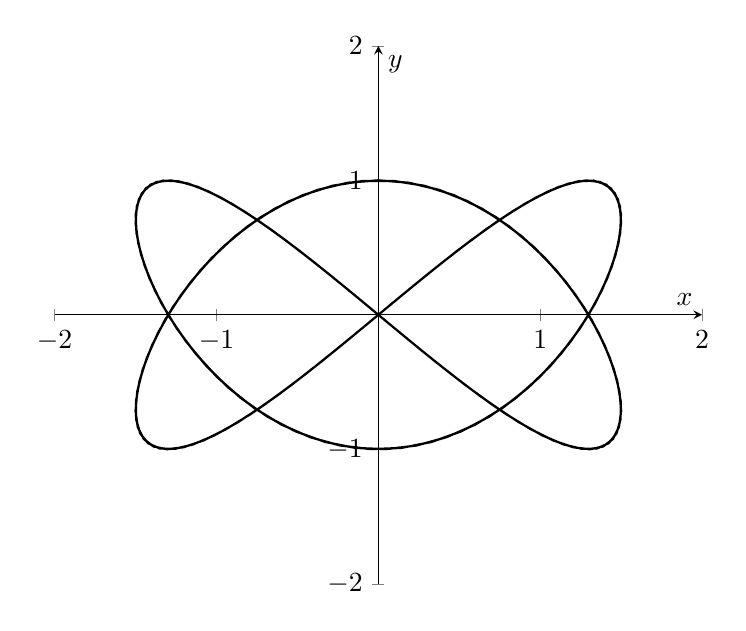
\begin{tikzpicture}
				\begin{axis}[
				scale=1.2,
				axis lines=center,%width=4cm,height=4cm,
				ymax=2,ymin=-2,
				xmax=2,xmin=-2,
				xtick={-2,-1,1,2},
				xlabel=$x$,ylabel=$y$,%	ytick=\empty,
				]
				\addplot[domain=0:4*360, samples=200, thick] ({-1.5*sin(x)},{cos(1.5*x)});
				\end{axis}
		\end{tikzpicture}
		}  \caption{Pokemon: $\displaystyle x=-\frac{3}{2}\sin(t),\,y=\sin\left(\frac{3t}{2}\right)$}
	\end{subfigure}
\end{figure}
To find the point at the mouth of the fish in terms of $t$, we must solve the equations for $x=-1.5$, or $y=0$. As $t$ increases, the plot is drawn.
\begin{equation*}
	\begin{aligned}[c]
x&=\frac{3\cdot\cos t}{2}\\
-1.5&=\frac{3\cdot\cos t}{2}\\
-1&=\cos t \\
t&=\pi\\
	\end{aligned}\qquad\qquad
	\begin{aligned}[c]
	 \text{check that }y&=0\\
	 y&=-\frac{2}{2}\cos\left(\frac{3\pi}{2}\right)\\
	y&=-\frac{2}{3}\cdot 0\\
	y&=0\\
	\end{aligned}
\end{equation*}
The point $t=0$ corresponds to $x=1.5$, and $y=-\frac{2}{3}=$ which is shown as a point on the tail.
\exercise In which direction is the Pokemon drawn? Where does it start?\\
\subsection*{Using the Chain Rule to find the Derivative $\frac{d y}{d x}$}
Given\ the parametric equations $x =f (t)$ and $y =g (t)$ define a parametric curve. If $f$ and $g$ are both differentiable the Chain Rule gives
\begin{equation*}\frac{d y}{d t} =\frac{d y}{\cancel{d x}} \cdot \frac{\cancel{d x}}{d t}
\end{equation*}

provided $y$ is also a differentiable function of $x$. So provided $\frac{d x}{d t} \neq 0$
\[\frac{d y}{d x} = \frac{d y}{d t} \div \frac{d x}{d t}\]
When dividing fractions remember to `invert and multiply'\\
\[\frac{d y}{d t} \times \frac{d t}{d x}=\frac{dy}{dx}\]

\example Find the derivative, $\frac{dy}{dx}$, of the fish in part (a).\medskip\\
\solution Differentiate each equation and combine with the chain rule to find $\frac{dy}{dx}$.\\
\begin{align*}x&=\frac{3\cos t}{2} &y=-\frac{2}{3}\cos\left({\frac{3t}{2}}\right)\\
\frac{dx}{dt}&=-\frac{3}{2}\sin t &\frac{dy}{dt}=-\frac{2}{3}\cdot-\sin \left({\frac{3t}{2}}\right)\cdot\frac{3}{2}\\
&&\frac{dy}{dt}=\sin \left({\frac{3t}{2}}\right)\\
\end{align*}
Now, using the chain rule, note $\frac{dx}{dt}$ must be inverted:\\
\begin{align*}\frac{dy}{dx}&=\frac{dy}{dt}\cdot\frac{dt}{dx}\\
&=\sin \left({\frac{3t}{2}}\right)\cdot \frac{1}{-\frac{3}{2}\sin t }\\
&=\frac{-2\sin \frac{3t}{2}}{3\sin t}
\end{align*}
Compare your derivatives, $y'$ and $x'$, with the superhero logo plot from part (b).
%---------------------------------------------------
% Related Rates
%---------------------------------------------------
\section{Related Rates}
The concept of related rates is best understood by exploring some examples.

\examq Air is being pumped into a spherical balloon so that its volume is increasing at a rate of 50 $cm^{3}$/$\mbox{s}$. How fast is the radius of the balloon increasing when the diameter is 50 $\mbox{cm}$? \\
\solution The volume of a sphere is $\frac{4}{3}\pi r^3$. Find the derivative with respect to radius.
\[\frac{d V}{d r} =4 \pi r^2\]
We are looking for ``how fast'' (time) and radius ($r$), or $\frac{dr}{dt}$. From the Chain Rule we can write
\[\frac{d V}{d t} =\frac{d V}{d r} \cdot \frac{d r}{d t}\]
Substituting $\frac{d V}{d t} =50$ and $\frac{d V}{d r} =4 \pi  r^{2}$ we get
\begin{align*}50 &  = 4 \pi  r^{2} \cdot \frac{d r}{d t} \\
\frac{d r}{d t} &  = \frac{50}{4 \pi  r^{2}} \\
\end{align*}
Now we substitute $r =25$. (Diameter $ =50$ so radius $ =25$)
\begin{align*}\frac{d r}{d t}_{r =25} &  = \frac{50}{4\pi(25)^2} \\
&  = \frac{1}{50 \pi }\approx 0.00637\end{align*}
Therefore the radius is increasing at the rate of $\displaystyle\frac{1}{50 \pi }$ cm/s.\\
\rule{6.8cm}{0.5pt}\\
\example A ladder $5$ $\mbox{m}$ long rests against a vertical wall. If the bottom of the ladder slides away from the wall at the rate of $0.5$ $\mbox{m}$/$\mbox{s}$ how fast is the top of the ladder sliding down the wall when the bottom of the ladder is $3$ $\mbox{m}$ from the wall?

\solution Let the origin be placed at the corner where the wall meets the floor, let $x$ be the distance of the foot of the ladder from the wall and let $y$ be the distance of the top of the ladder from the corner. The ladder forms a right angled triangle whose sides are $x$, $y$ and with hypotenuse $5$. We are given that $\frac{d x}{d t} =0.5$ and are asked to find $\frac{d y}{d t}$ when $x =3$.

Pythagoras' theorem gives
\begin{equation}x^{2} +y^{2} =5^{2}\tag{1}
\end{equation}

Differentiate equation (1) with respect to $t$. Note that this derivative uses a technique called implicit differentiation.
\begin{equation*}2 x \frac{d x}{d t} +2 y \frac{d y}{d t} =0
\end{equation*}

Solve for $\frac{d y}{d t}$
\begin{equation*}\frac{d y}{d t} = -\frac{x}{y} \cdot \frac{d x}{d t}
\end{equation*}

Using the Pythagorean theorem with $x=3$ and the hypotenuse $=5$, $y=4$

Substitute $\frac{d x}{d t} =0.5$, $x =3$ and $y =4$
\begin{align*}\frac{d y}{d t} &  =  -\frac{3}{4} \cdot 0.5 \\
 &  =  -0.375\end{align*}

The top of the ladder is moving vertically downwards at the rate of 0.375 m/s.\\
\rule{6.8cm}{0.5pt}\\
\example A water tank has the shape of an inverted circular cone with a base radius of $2$ $\mbox{m}$ and height of $4$ $\mbox{m}$. If water is being pumped into
the tank at a rate of $2$ $\mathrm{m}^{3}$/$\mbox{min}$ find the rate at which the water level is rising when the water is $3$ $\mbox{m}$ deep.

\begin{multicols}{2}
\solution Let $V$, $r$ and $h$ be the volume of water the radius of the surface and the height at time $t$. We are given
\begin{equation*}\frac{d V}{d t} =2\text{}\mathrm{m}^{3}/\mbox{min}
\end{equation*}

We are asked to find $\frac{d h}{d t}$ when $h =3$.

Draw a diagram to show that the relationship between $r$ and $h$ can be found by similar triangles.
\begin{align}\frac{r}{h} &  = \frac{2}{4} \nonumber  \\
r &  = \frac{h}{2} \tag{1}\end{align}

The formula for the volume is
\begin{equation}V =\frac{1}{3} \pi  r^{2} h\tag{2}
\end{equation}

Substituting equation (1) in equation (2)
\begin{align*}V &  = \frac{1}{3} \pi  \genfrac{(}{)}{}{}{h}{2}^{2} h \\
 &  = \frac{\pi }{12} h^{3}\end{align*}

Differentiate with respect to $t$
\begin{align*}\frac{d V}{d t} &  = \frac{\pi }{12} \cdot 3 h^{2} \cdot \frac{d h}{d t} \\
 &  = \frac{\pi }{4} h^{2} \cdot \frac{d h}{d t}\end{align*}

So
\begin{equation*}\frac{d h}{d t} =\frac{4}{\pi  h^{2}} \cdot \frac{d V}{d t}
\end{equation*}

Substitute $h =3$ and $\frac{d V}{d t} =2$
\begin{align*}\frac{d h}{d t} &  = \frac{4}{\pi  \left (3\right )^{3}} \cdot 2 \\
 &  = \frac{8}{9 \pi }\end{align*}

The water level is rising at the rate of $\frac{8}{9 \pi }$ $\mbox{m}$/$\mbox{min}$.
\end{multicols}


%---------------------------------------------------
% Optimisation
%---------------------------------------------------
\section{Optimisation}\label{sec:Optimisation}
Optimisation is the process of using calculus to find the best result for a situation involving a changing quantity (variable). Examples include  maximizing profit, minimizing cost, maximizing volume, minimizing amount materials used, and so on. As long as the quantities in question can be represented by a function, calculus can used to find the special points of the function and their nature.

\begin{tcolorbox}
	A general method to approach an optimisation problem
	\begin{enumerate}
		\item Write down the known variables and draw a diagram
		\item Form an equation of the situation by placing the unknown variable in terms of the known variables
		\item Use the facts of the problem to reduce the expression until it becomes a relationship between the unknown quantity and one of the known quantities
		\item Optimize by finding a maximum or minimum value
	\end{enumerate}
\end{tcolorbox}

%Example level: EASY
\example A farmer wishes to fence a paddock using an existing wall as one side of the paddock. She has 100 meters of fencing and wants to know the dimensions of the paddock to enclose the maximum area.
% include the plot file for
% optimisation paddock
\begin{center}
	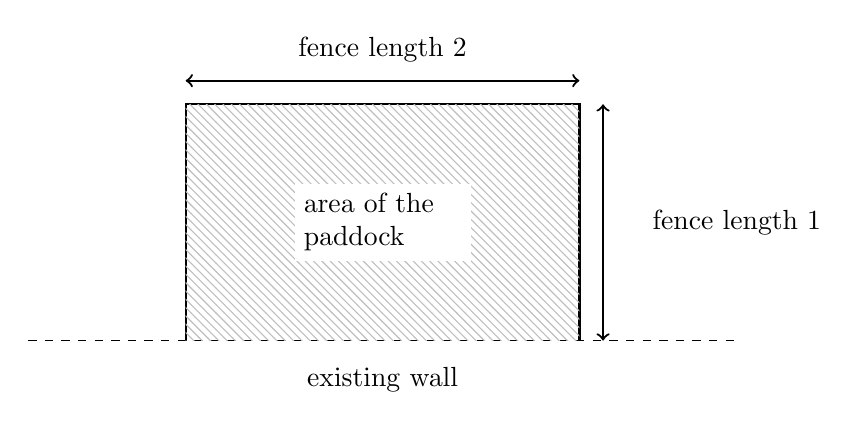
\begin{tikzpicture}
	\usetikzlibrary{patterns}
	\draw [thick](0,0) -- (0,3) -- (5,3) -- (5,0);
	\draw [dashed](-2,0) -- (7,0);
	\draw[pattern=north west lines, pattern color=gray!50, draw=none] (0,0) rectangle (5,3);
	\node at (2.5,-0.5) {existing wall};
	\draw [<->,thick] (5.3,0)--(5.3,3);
	\node at (7,1.5){fence length 1};
	\draw [<->,thick] (0,3.3)--(5,3.3);
	\node at (2.5,3.7){fence length 2};
	\node [text width=2cm, fill=white]at (2.5,1.5){area of the paddock};
	\end{tikzpicture}
\end{center}
\solution Following the steps outlined above, draw a diagram and label the variables. Let $T$ represent the total fence length which cannot be more than 100m. Write this as an equation: $T=100$. There are 3 individual lengths that make up the total, so let $l$ represent the long side of the paddock, and $w$ represent the short side.
\begin{align*}
T&=l+2w\\
100&=l+2w
\end{align*}
The quantity to be optimised is area ($A$) of the paddock (remember it is a rectangle):
\begin{align*}
A=lw
\end{align*}
The next step is to represent the quantity to be optimised (area) as a function of one other variable. We can rearrange our earlier equation to solve for length: $l=100-2w$. This can now be substituted into the area equation:
\begin{align*}
A&=lw\\
&=\left(100-2w\right)w\\
&=100w-2w^2
\end{align*}
This is now an equation that can optimised using calculus.
\begin{align*}
\frac{dA}{dw}&=100-4w\\
0&=100-4w\\
w&=25
\end{align*}
Therefore the paddock width is 25 meters to maximize the total area. Going back to the original constraint of 100m total length means that the paddock length is $100-2(25)=50$ meters.\\
\rule{6.8cm}{0.5pt}\\
%Example level: EASY
\example A cylindrical can is to be made to hold 1 litre of oil. Find the dimensions that will minimise the cost of the aluminium to manufacture the can. Note that 1 L = 1000 cm$^3$.\\

\begin{figure}[h]
	\centering
	\begin{subfigure}[h]{0.4\textwidth}
		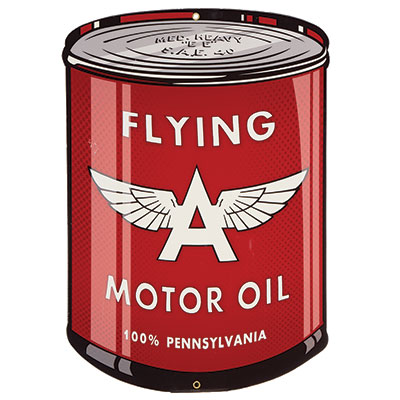
\includegraphics[width=\textwidth]{graphics/oilCan}
	\end{subfigure}
	\begin{subfigure}[h]{0.4\textwidth}
		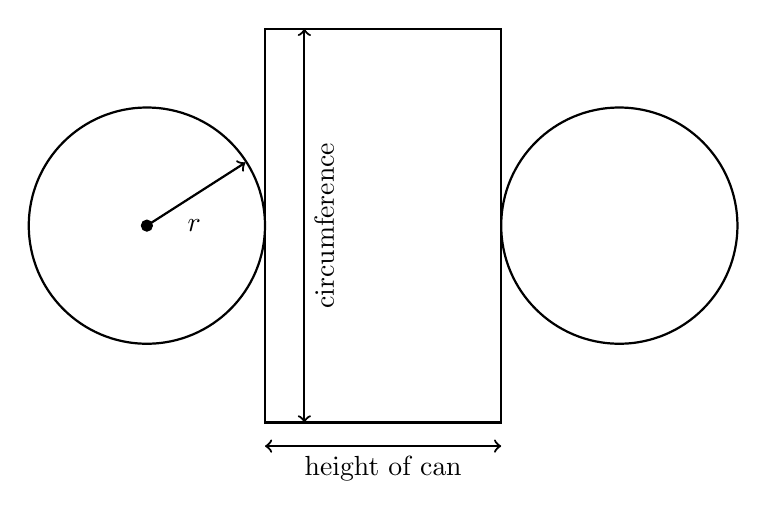
\begin{tikzpicture}
		\draw [thick](0,-1)rectangle(3,4);
		\draw [<->,thick] (0,-1.3)--(3,-1.3) node[below,xshift=-1.5cm]{height of can};
		\draw [<->,thick] (0.5,-1)--(0.5,4) node[below,yshift=-2.5cm,rotate=90]{circumference};
		\draw [thick](-1.5,1.5) circle [radius=1.5];
		\draw [thick](4.5,1.5) circle [radius=1.5];
		\draw[->,thick](-1.5,1.5)--(-0.25,2.3);
		\node at (-.9,1.5){$r$};
		\filldraw (-1.5,1.5) circle (2pt) ;
		\end{tikzpicture}
	\end{subfigure}
\end{figure}

\solution The minimum cost of the aluminium will be the minimum surface area of the cylinder. The can can be deconstructed into two circles and a rectangle. We will label the variables required to calculate area.

Let $SA$ represent surface area of the can. The total surface area is:
\begin{align*}
SA&=\pi r^2 + \pi r^2 + \left(\textrm{height}*\textrm{circumference}\right)\\
&=2\pi r^2+2\pi rh
\end{align*}
Note that we have 2 variables that are unknown, $r$, and $h$. We need to express one variable in terms of the other in order to proceed. Use the additional information in the problem. The volume of the can must be 1000 cm$^3$.
\begin{multicols}{2}
\begin{align*}
V&=\pi r^2 h\\
1000&=\pi r^2 h\\
h&=\frac{1000}{\pi r^2}
\end{align*}
Substitute this form for $h$ into the surface area function:
\begin{align*}
\text{SA}&=2\pi r^2+2\pi rh\\
&=2\pi r^2+2\pi r\left(\frac{1000}{\pi r^2} \right)\\
&=2\pi r^2+\frac{2000}{r}
\end{align*}
This function is now the surface area in terms of a single variable, $r$, and can be optimised:
\begin{align*}
\frac{d(\text{SA})}{dr}&=4\pi r-\frac{2000}{r^2}\\
0&=4\pi r-\frac{2000}{r^2}\\
&=4\pi r^3-2000\\
r^3&=\frac{2000}{4\pi}\\
r&=5.419 \,\textrm{cm}
\end{align*}
Therefore the final dimensions of the can optimised for minimum cost are radius$=5.42$ cm, and height$=10.8$ cm.
\end{multicols}




%---------------------------------------------------
% Chapter Exercises in a separate file
%---------------------------------------------------
% \clearpage
 \section{Chapter Exercises}
 \subimport{}{4DifferentiationExercises}
